\documentclass[12pt]{amsart}
\usepackage{amsaddr}
\usepackage{marktext} 
%% Remove draft for real article, put twocolumn for two columns
\usepackage{svmacro}
\usepackage[utf8]{inputenc}
\usepackage[style=alphabetic, backend=biber]{biblatex}
\addbibresource{bibliography.bib}

%% commentary bubble
\newcommand{\SV}[2][]{\sidenote[colback=green!10]{\textbf{SV\xspace #1:} #2}}

%% Title 
\title{ Calculus }
\author{  Final B \\ \vspace{1cm} Name: \_\_\_\_\_\_\_\_\_\_\_\_\_\_\_\_\_\_\_\_\_\_\_\_\_  
\\ \vspace{1cm} ID: \_\_\_\_\_\_\_\_\_ \\ \vspace{1cm} Score: \_\_\_\_\_\_/ 100}

\date{\today}

\begin{document}

\maketitle


RULES:
\begin{itemize}
	\item You have 80 minutes to complete the exam.
	\item There are 5 questions and 100 points in total.
	\item You can use a non-graphing calculator.
	\item If you need to go to the restroom, please turn in your cellphone before.
	\item If you need hints, 1 hint is worth 3 points.
\end{itemize}

\newpage

\begin{problem}[20 points]
\begin{enumerate}
	\item How many kinds of discontinuity are there? Draw graphs to demonstrate.
	      \vspace{11cm}

	\item State one out of two parts of the fundamental theorem of calculus? Just pick one.
	      \vspace{11cm}

	      \newpage
	\item State the L'Hospital rule.
	      \vspace{11cm}

	\item Define the left-end Riemann sum for a continuous function $f(x)$ on the interval $[a,b]$.
	      \vspace{11cm}
\end{enumerate}
\end{problem}

\newpage

\begin{problem}[20 points]
Compute the following:

\begin{enumerate}
	\item $$ \lim_{x \to 1^+} \frac{ e^{\sin(x-1)-1} - 1}{\ln(x-1)} $$
	      \vspace{8cm}
	\item $$ \frac{d}{dx} \left( \sin (e^x) e^{\cos (x)}  \right)$$
	      \vspace{8cm}
	\item $$ \int_0^\pi \sin(2x) e^x \, dx $$
	      \vspace{8cm}

	\item $$\int  x\sqrt{x^2-1} \, dx $$
	      \vspace{8cm}

\end{enumerate}
\end{problem}

\newpage

\begin{problem}[20 points]
\begin{enumerate}
	\item What is the chain rule?
	      \vspace{5cm}
	\item Find $y'(\pi)$ where
	      \begin{equation*}
		      \tan(xy) = y \,,
	      \end{equation*}
	      and $y(\pi)= 1$.
\end{enumerate}
\end{problem}

\newpage

\begin{problem}[20 points]

Two poles are connected by a wire that is also connected to the ground. The first pole is $20 \, \text{ft}$ tall, and the second pole is $10 \, \text{ft}$ tall. There is a distance of $30 \, \text{ft}$ between the two poles. Where should the wire be anchored to the ground to minimize the amount of wire needed?

\begin{figure}[ht!]
	\begin{center}
		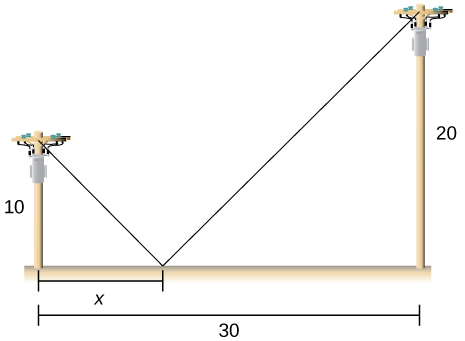
\includegraphics[width=0.7\textwidth]{drones.jpeg}
	\end{center}
\end{figure}


\end{problem}

\newpage

\begin{problem}[20 points]
Use the method of shells to find the volume of a cone with radius $r$
and height  $h$.

\begin{figure}[ht!]
	\begin{center}
		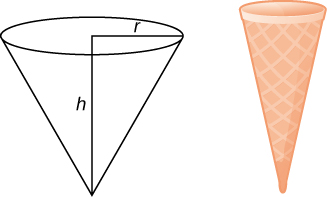
\includegraphics[width=0.7\textwidth]{cone2}
	\end{center}
\end{figure}


\end{problem}


\end{document}
